
% This LaTeX was auto-generated from MATLAB code.
% To make changes, update the MATLAB code and republish this document.

\documentclass{article}
\usepackage{graphicx}
\usepackage{color}

\sloppy
\definecolor{lightgray}{gray}{0.5}
\setlength{\parindent}{0pt}

\begin{document}

    
    \begin{verbatim}
Ra = 10;
La = 5;
Ke = 0.02;
Kt = 0.4;

N1 = 44;
N2 = 38;
N3 = 38;
N4 = 24;

J = 0.002;

c1 = 240;
c = c1;
c3 = c1;

k1 = 3500;
k2 = 3500;

t = 0:0.01:5;
va = 100*sin(60*t);
ml = 200*sin(10*t);

s = tf('s')
%syms s

a11 = J*s^2 + c*s + k1 + k2 - k1^2/((N1/N1)^2 *c1*s + k1) - k2^2/((N3/N4)^2*c3*s + k2);

a12 = -(k1*Kt)/((N2/N1)*c1*s + (N2/N1)*k1);

a21 = (Ke*k1*s)/((N2/N1)*c1*s + (N1/N2)*k1);

a22 = La*s + Ra + (Ke*Kt*s)/(c1*s + (N1/N2)^2*k1);

b = -k2/((N3/N4)*c3*s + (N4/N3)*k2);


G = inv([a11/b, a12/b; a21, a22]);
s = tf('s');

G11 = G(1,1)
G12 = G(1,2)


theta = lsim(G11,ml,t) + lsim(G12,va,t);

omega = diff(theta)/0.01;  % Finite difference approx derivative
plot(t(1:length(omega)),omega)
box on
grid on
xlabel('Time [seconds]')
ylabel('Midshaft velocity [rad/s]')
title('Q10.3 Midshaft Velocity')
\end{verbatim}

        \color{lightgray} \begin{verbatim}
s =
 
  s
 
Continuous-time transfer function.


G11 =
 
                                                                          
  -4605 s^6 - 3.504e05 s^5 - 1.05e07 s^4 - 1.558e08 s^3 - 1.168e09 s^2    
                                                                          
                                                    - 3.97e09 s - 4.356e09
                                                                          
  ------------------------------------------------------------------------
                                                                          
  s^9 + 1.201e05 s^8 + 1.333e07 s^7 + 5.778e08 s^6 + 1.269e10 s^5         
                                                                          
          + 1.512e11 s^4 + 9.59e11 s^3 + 2.894e12 s^2 + 2.976e12 s        
                                                                          
                                                               - 0.0006996
                                                                          
 
Continuous-time transfer function.


G12 =
 
                                                                           
  -1.264e-13 s^7 - 1.514e-08 s^6 + 675.4 s^5 + 4.412e04 s^4 + 1.088e06 s^3 
                                                                           
                                    + 1.248e07 s^2 + 6.558e07 s + 1.274e08 
                                                                           
  -------------------------------------------------------------------------
                                                                          
  s^9 + 1.201e05 s^8 + 1.333e07 s^7 + 5.778e08 s^6 + 1.269e10 s^5         
                                                                          
          + 1.512e11 s^4 + 9.59e11 s^3 + 2.894e12 s^2 + 2.976e12 s        
                                                                          
                                                                - 0.003562
                                                                          
 
Continuous-time transfer function.

\end{verbatim} \color{black}
    
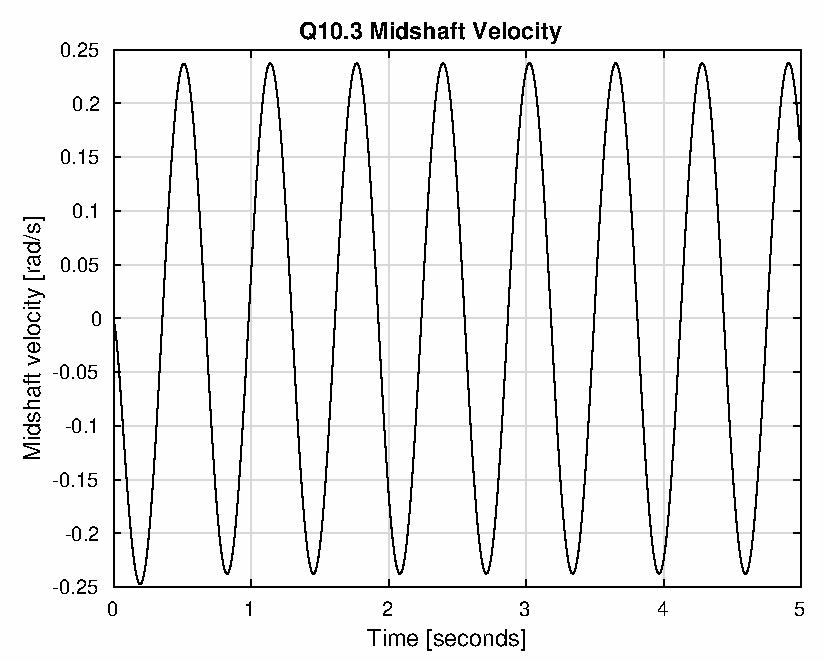
\includegraphics [width=4in]{Q10_3_01.eps}



\end{document}
    
